\section{System Overview}

\subsection{Use Cases}
Figure \ref{fig:pi-use-cases} shows a general overview of the use cases we have included in our prototype. A medication process can be started in one out of two ways. 
A parent can register an alarm by using AsthmAPP. This alarm is then triggered by AsthmaBuddy, giving the child a notification that it is time to take their medicine.

The alternative is if children need to take their medicine by need. If they need to take a medicine by need, they simply register their RFID-tag before children are taken through a quicker process (see Manuscript \ref{chp:anuscript}).  

\begin{figure}[H] 
	\centering
		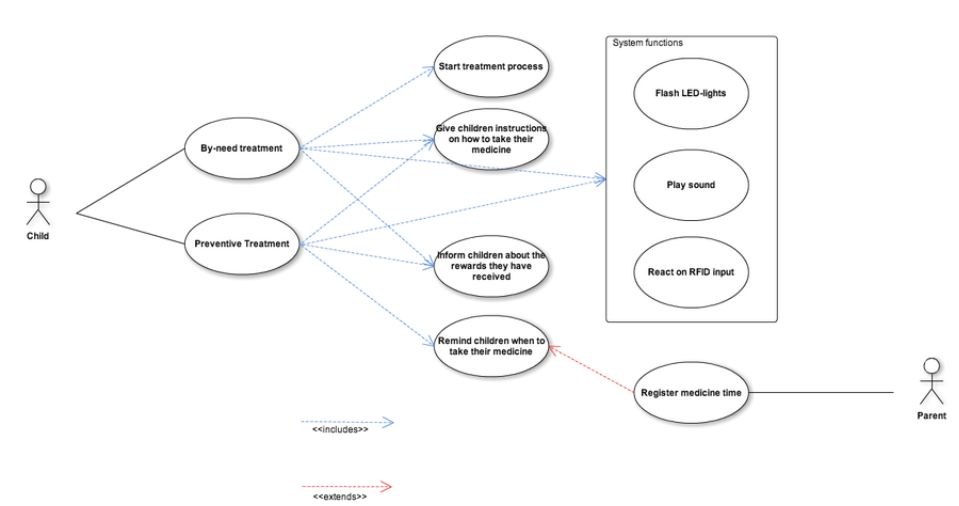
\includegraphics[width=0.8\paperwidth]{Pictures/usecases.png}
	\caption{AsthmaBuddy Use Cases}
	\label{fig:pi-use-cases}
\end{figure}

\subsection{Textual Use Cases}

%--------- TEXTUAL USE CASE ----------
%--------- BY NEED TREATMENT ---------
\begin{table}[H]
\begin{tabular}{|p{4.0cm} | p{9.0cm} |}
\hline
\textbf{Title} & By need treatment \\
\hline
\textbf{Preconditions} & - \\
\hline 
\textbf{Scenario} & 
	\begin{enumerate}
	  \itemsep0em
	  \item User triggers treatment by holding a specific RFID-tag close to AsthmaBuddy
	  \item System flashes LED-lights to notify user that the system is ready for use
	  \item System plays sound to instruct the user to shake the medicine
	  \item System plays sound to instruct user to mount the medicine on the mask and place the mask on his/her face
	  \item User starts a treatment by interacting with AsthmaBuddy (by pressing it's hand or similar interaction)
	  \item System plays sound to count during treatment (1-2-3-4-5-6-7-8-9-10), while flashing lights for each count
	  \item System plays sound to tell user he/she has done a good job
	  \item System calculates reward based on health state
	  \item System plays sound to award user with the calculated amount of stars
	  \item System plays sound to tell the user how many stars he/she has collected totally
	\end{enumerate}
\\
\hline
	\textbf{Extensions} & 
		x.a User aborts treatment by not continuing the sequence
\\
\hline
\end{tabular}
\caption{Textual use case: By need treatment}
\label{tab:textual-use-case}
\end{table}


%--------- PREVENTIVE TREATMENT -------

\begin{table}[H]
\begin{tabular}{|p{4.0cm} | p{9.0cm} |}
\hline
\textbf{Title} & Planned treatment \\
\hline
\textbf{Preconditions} & The current time corresponds with the time for a planned treatment \\
\hline 
\textbf{Scenario} & 
	\begin{enumerate}
	  \itemsep0em
	  \item The system recognizes the time for a planned treatment
	  \item The system starts blinking with LED-lights and playing sound to notify user
	  \item Child registers interacts with AsthmaBuddy, to notify that he/she is ready for the treatment
	  \item Start instructions by playing sound, telling the user to find a grown-up that can keep watch
	  \item System waits for interaction to make sure the user is ready
	  \item System tells the user to mount the medicine on the mask and put the medicine towards AsthmaBuddy's face
	  \item System plays sound to simulate breathing
	  \item System plays sound to tell the user how easy it was to take medicines and that it is the user's turn
	  \item System plays sound to instruct user, telling the user to shake the medicine
	  \item System waits for interaction to make sure the user is ready
	  \item System plays sound to instruct user to put the mask on his/her face
	  \item System plays sound counting to 10. 
	  \item System plays sound to tell the user he/she has done a good job
	  \item System calculates reward based on health state
	  \item System plays sound to award user with the calculated amount of stars
	  \item System makes a HTTPGet call to the server to find the total amount of stars collected
	  \item System plays sound to inform the user about how many stars the user has collected totally
	\end{enumerate}
\\
\hline
	\textbf{Extensions} & 
		x.a Child does not interact with AsthmaBuddy when prompted
\\
\hline
\end{tabular}
\caption{Textual use case: By need treatment}
\label{tab:textual-use-case}
\end{table} 


\subsection{State Diagram}
When the \rpi{} boots, it retrieves the latest version of the source code from Git, compiles it, and starts running it. If a child approaches \buddy{} and registers a RFID-tag, a medication sequence is started.  

\begin{figure}[H] 
	\centering
		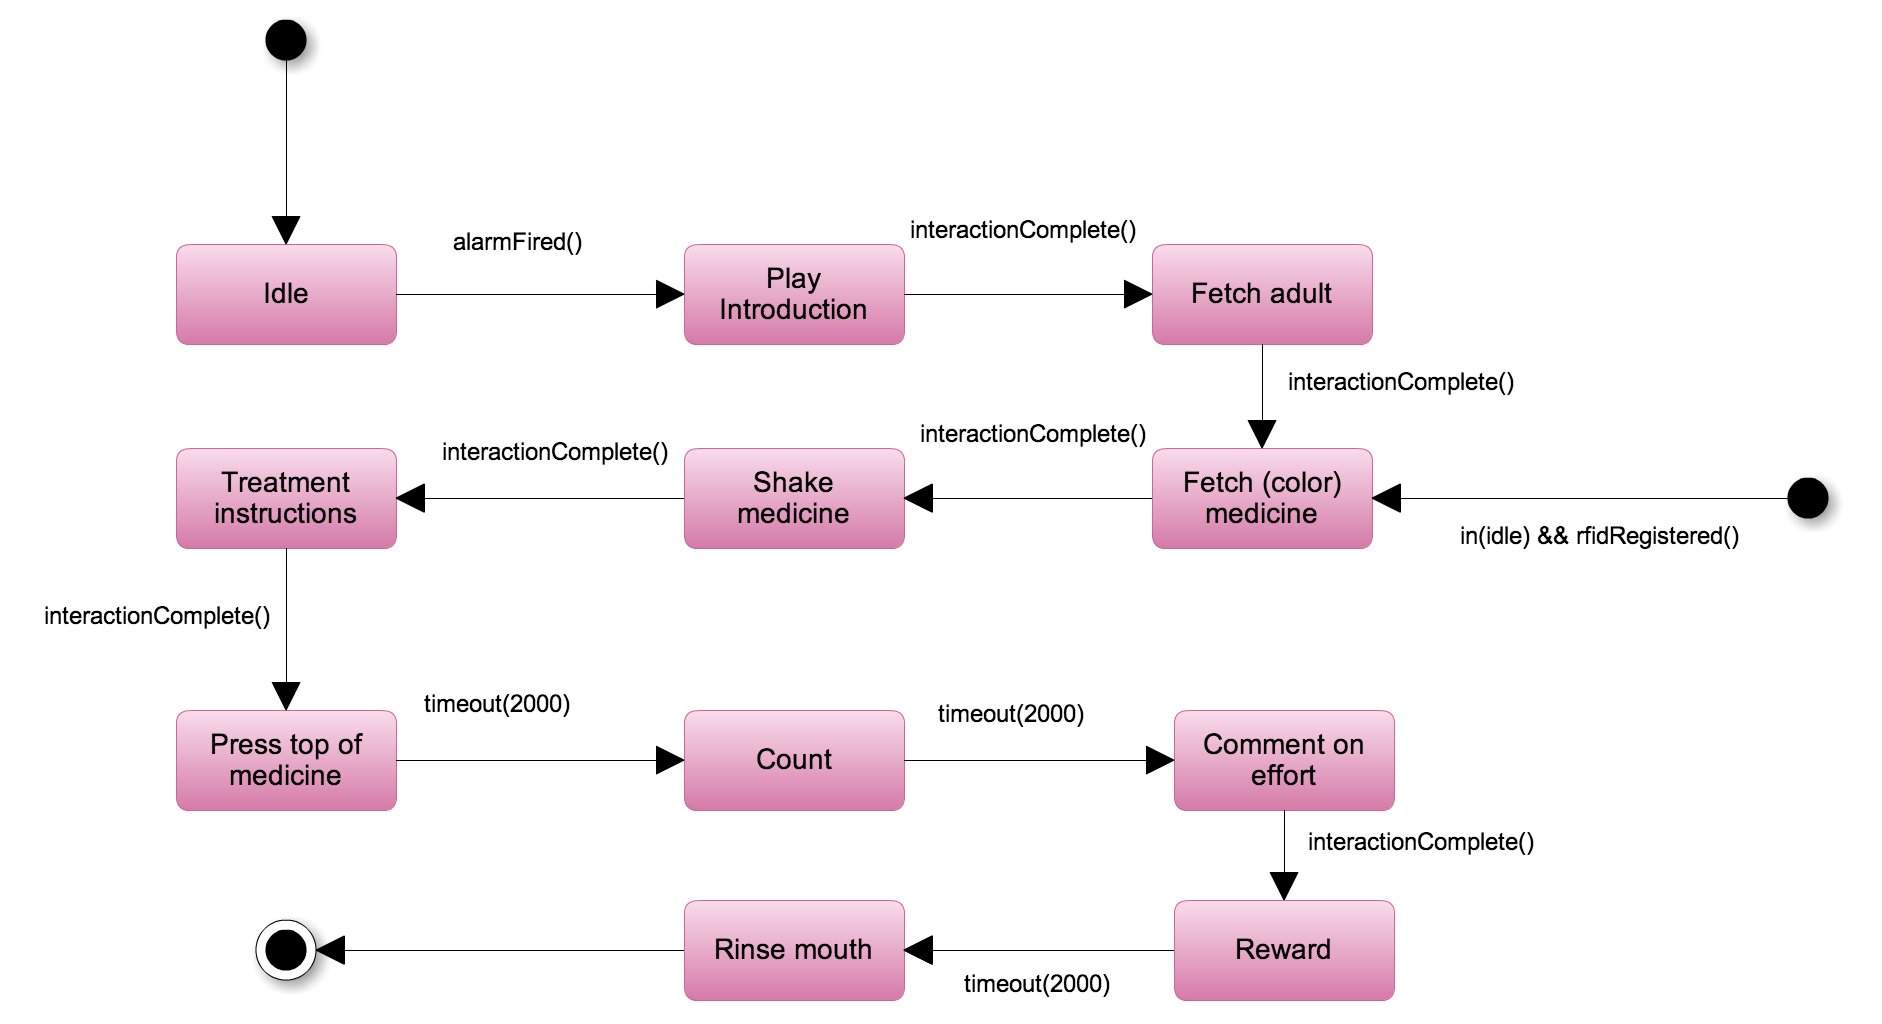
\includegraphics[width=0.6\paperwidth]{Pictures/statediagram.png}
	\caption{AsthmaBuddy State Diagram.}
	\label{fig:asthmabuddy_statediagram}
\end{figure}

\subsection{Sequence Diagram}
Figures \ref{fig:ab-sd-byneed} - \ref{fig:ab-sd-completing-treatment} shows sequence diagrams of how the system works internally. Some abstractions have been made, in order to reduce the cluster of arrows. 

\subsubsection{By Need Treatment}

\subsubsection{Planned Treatment}

\subsubsection{Playing Instructions}

\subsubsection{Finishing a Treatment}



\begin{sidewaysfigure}
	\centering
		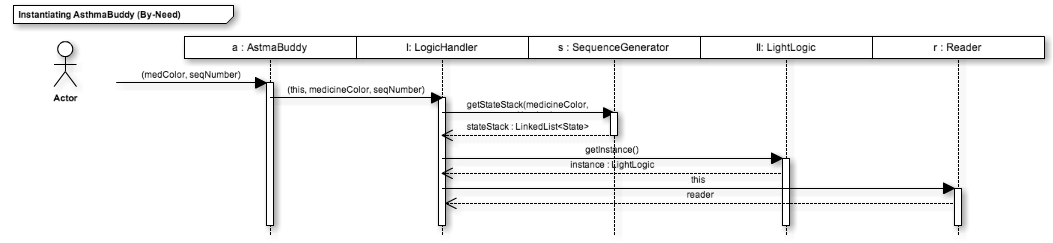
\includegraphics[scale=0.6]{Pictures/sd/sd-byneed.png}
	\caption{By Need Treatment - Sequence Diagram}
	\label{fig:ab-sd-byneed}
\end{sidewaysfigure}

\begin{sidewaysfigure}
	\centering
		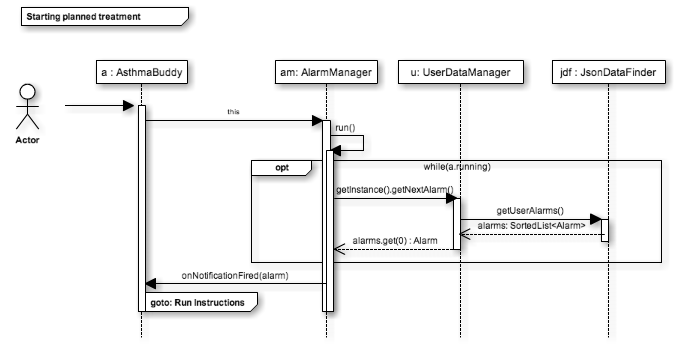
\includegraphics[scale=0.6]{Pictures/sd/sd-planned-treatment.png}
	\caption{Planned Treatment - Sequence Diagram}
	\label{fig:ab-sd-planned-treatment}
\end{sidewaysfigure}

\begin{sidewaysfigure}
	\centering
		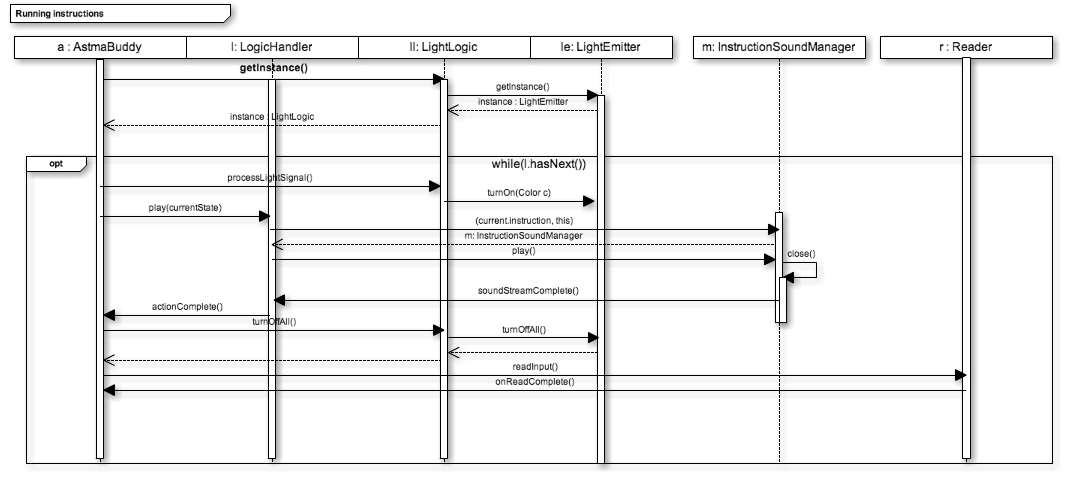
\includegraphics[scale=0.6]{Pictures/sd/sd-instructions.png}
	\caption{Playing Instructions - Sequence Diagram}
	\label{fig:ab-sd-instructions}
\end{sidewaysfigure}

\begin{sidewaysfigure}
	\centering
		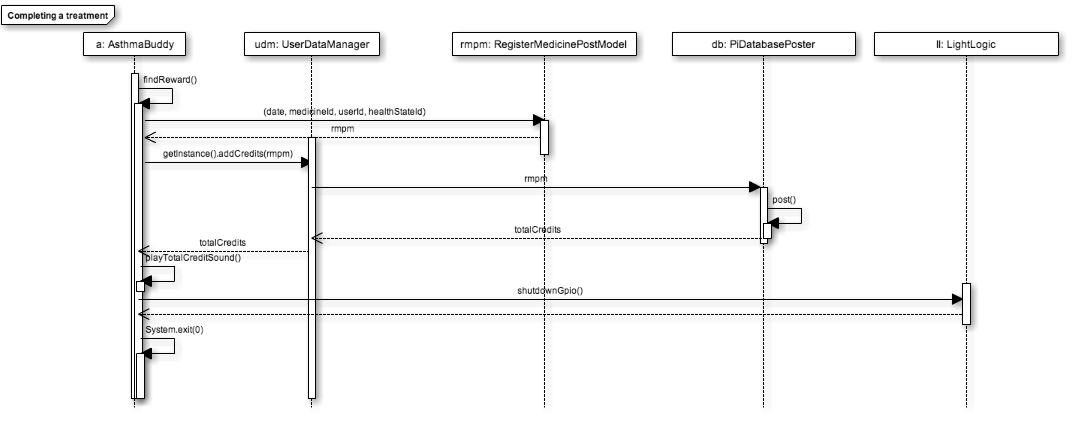
\includegraphics[scale=0.6]{Pictures/sd/sd-complete-treatment.png}
	\caption{Finishing a treatment - Sequence Diagram}
	\label{fig:ab-sd-completing-treatment}
\end{sidewaysfigure}

\subsection{Node Server}
In addition to the Java application running on the \rpi{}, we developed a Node.js server\fnurl{Node.js}{http://nodejs.org/}. This backend system was developed in order to easily visualize the rewards given to a child. The initial problem is that AsthmAPP stores data to a MySQL database, with childId as the primary key for most tables. Initially, \buddy{} has no way of knowing which childId to use in order to store the rewards. The current solution to our problem was to develop a Node.js server on AsthmaBuddy, which run as a background process. Whenever we want to switch users, AsthmAPP does an HTTP POST to this server, including the childId as a parameter. The server then retrives JSON-formatted data from a webservice, which includes the rewards a child has been given until now (for instance, by use of the smartphone), and the alarms set for this user. 
When \buddy{} starts running, it checks for alarms to be fired every 60 seconds. When a child has finished a treatment, AsthmaBuddy updates the database, with the childId previously retrieved, and the amount of stars a child gathered during his or her treatment. Additionally, with the data retrieved from the database, \buddy{} has the capability to tell the user how many stars a child has gathered\footnote{Since this is a prototype, this functionality only works until a child has gathered 20 stars. It became cumbersome to handle rewards totalling more than 20 stars}. 

